\documentclass[12pt,a4paper]{article}
\usepackage[utf8]{inputenc}
\usepackage[english]{babel}
\usepackage{amssymb}%usar formula matematica
\usepackage{graphicx}%insere imagem
\usepackage{wrapfig}
\usepackage{float}
\usepackage{hyperref}
\usepackage{indentfirst}
\usepackage{enumitem}
\usepackage{amsmath}
\usepackage{booktabs}
\usepackage{cancel}
\usepackage{subfig}
\usepackage{siunitx}
\usepackage[alf]{abntex2cite} 
%\newtheorem{teo}{Teorema}
\renewcommand{\baselinestretch}{1.5}%estilo da fonte
\usepackage{verbatim} % para comentarios
\usepackage{float}  % para imagens
\usepackage{xcolor}
\usepackage{listings}
\usepackage{geometry}%configura margem
%\geometry{verbose,a4paper,tmargin=30mm,bmargin=20mm,lmargin=30mm,rmargin=20mm}

\begin{document}
\newgeometry{top = 1.5cm, lmargin = 1.5cm, rmargin = 1.5cm} 

\begin{figure}[H]
	\centering
	\begin{minipage}[]{0.07\linewidth}
	
\includegraphics[width=\linewidth]{images/ufop.png}	
	\end{minipage}
\hfill
	\begin{minipage}[]{0.6\linewidth}
		\centering
	\textbf{UNIVERSIDADE FEDERAL DE OURO PRETO\\}
		Rafael Francisco de Oliveira - 2021.10171\\
		PCC104 - Projeto e Análise de Algoritmos\\
		Github: \href{https://github.com/raffoliveira/Master_Degree}{raffoliveira}\\
		Lista 1
		
	\end{minipage}
\hfill	
	\begin{minipage}[c]{0.15\linewidth}
	
\includegraphics[width=\linewidth]{images/icea.jpg}	
	\end{minipage}

\vspace{0.5cm}
\hrulefill
\end{figure}

\begin{enumerate}
	\item Por que estudamos algoritmos?
	
	Há várias razões para o estudo de algoritmos. Primeiramente, se o objetivo do estudo for se tornar um profissional da computação há os motivos prático e teórico deste estudo. No ponto de vista prático, permite uma visão ampla de importantes algoritmos em diferentes áreas dentro da computação permitindo a criação de novos algoritmos e análise de melhor eficiência entre eles. No ponto de vista teórico, o estudo ajuda entender a importância dos algoritmos para a ciência da computação como sendo o ponto principal. Fora do objetivo profissional, hoje praticamente tudo envolve o uso de tecnologia e consequentemente o uso de computadores e suas aplicações. Portanto, mesmo que o objetivo não seja ser expert em computação, o conhecimento de algoritmo com certeza facilitará a usabilidade dessa ferramenta tão essencial. Outra razão temos o desenvolvimento de habilidades analíticas que auxiliam na resolução de problemas e estratégias de solução.	
	
	
	\item O que é um algoritmo?
	
	A especificação do que é um algoritmo é muito ampla, mas resumidamente seria um conjunto de sequência de instruções bem definidas e sem ambiguidade a serem seguidas, passo a passo, para fazer algo em específico ou resolver algum tipo de problema, dado uma determinada entrada e um tempo finito de solução.
	
	
	\item Considere o algoritmo de
	\href{https://en.wikipedia.org/wiki/Euclidean_algorithm#Implementations}{Euclids} para o cálculo do maior divisor comum. Como sabemos que este termina em	tempo finito?
	
	Dado o algoritmo $gcd(m,n)$, $n = 0$ é o critério de parada, fazendo com que o algoritmo pare quando chegar nesse valor. E pelo algoritmo de Euclides, a cada iteração, o valor de $n$ é atualizado com ($m$ mode $n$), o que é sempre menor que $n$ (por ser o resto de uma divisão), fazendo com que chegue a zero depois de algum tempo.
	
	
	
	\item Considere os procedimentos para o cálculo do maior divisor comum. Por que este procedimento não se qualifica como um algoritmo legítimo?
	
	Pela definição de algoritmo, temos que é necessário ter instruções bem definidas e sem ambiguidade para qualificarmos como algoritmo. Nos passos 1 e 2, pede-se para encontrar os números primos de $m$ e $n$, mas não diz como se faz isso. Enquanto não se resolve esse problema não é possível seguir os procedimentos. Ou seja, temos um problema dentro de um algoritmo que resolve outro algoritmo. Logo, as instruções não deixaram claro como se faz cada passo, abrindo margem para ambiguidade e não mal definição.
	
	
		
	\item O que diferencia a ciência da computação da matemática?
	
	Ambos usam algoritmo e modelos para analisar dados. Na ciência de computação, os algoritmos são utilizados para executar específicas tarefas afim de solucionar algum problema, ou aumentar a eficiência dos computadores. Por outro lado, na matemática, os algoritmos são utilizados para pesquisar teorias matemáticas e desenvolver provas sobre a existência de soluções e analisar suas propriedades.
	
	
		
	\item Ilustre, com um fluxograma, o processo de projeto de análise de algoritmos e apresente uma pequena explicação sobre cada passo.
	
	\begin{figure}[H]
		\centering
		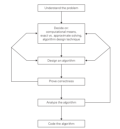
\includegraphics[scale=5]{images/algorithm_design.pdf}
		\caption{Fonte: \cite{levitin2008introduction}}
	\end{figure}

	\textit{Understand the problem}: entender completamente o problema em questão. Criar perguntas sobre, tipos de entradas, pensar em casos especiais fazem parte deste passo. Caso o problema em questão tem já algoritmos desenvolvidos, pode-se iniciar o processo de avaliação de algoritmos, suas eficiências e fraquezas, pois provavelmente será necessário recriar um novo algoritmo.
	
	\textit{Algorithm design technique}: nessa parte preocupa-se com a capacidade computacional que o algoritmo requer. Se o algoritmo faz uso apenas de processamento em RAM, pode ser executado em operação concorrentes (paralelas), tempo é crucial na execução, qual tipo de paradigma a ser utilizado, a solução será exata ou aproximada são algumas questões que devem ser respondidas. Essa parte permite a classificação do algoritmo dentro da ciência.
	
	\textit{Design an algorithm}: aqui desenvolve em si o algoritmo de acordo com a técnica escolhida. Muita das vezes é necessário combinar técnicas e escolhas de melhores estruturas de dados para melhor performance.
	
	\textit{Prove correctness}: agora é necessário provar se o algoritmo está correto, analisando os resultados de acordo com a entradas. Normalmente faz uso de indução matemática para tal. A falha é mais fácil de ser verificada. No caso de algoritmo por aproximação, a prova é feito a partir de um erro aceitável dentro de um limite pré-definido. Em caso de falha, é preciso voltar na parte da decisão de técnicas a serem utilizadas e reescrever o algoritmo novamente.
	
	\textit{Analyse the algorithm}: analisa-se a eficiência (tempo e espaço), simplicidade e generalidade do algoritmo. Novamente, caso haja algum desses fatores que podem ser melhorados, volta-se ao passo de escolha de técnicas e reescrita do algoritmo.
	
	\textit{Code the algorithm}: finalmente chegando nesse passo, pode-se codar o algoritmo, ou seja, torná-lo um programa que possa ser executado por uma máquina, realizando os testes e debugs do mesmo.
	
	
	
	\item Indique como a estrutura de dados abstrata, Fila de Prioridade pode ser implementada com as seguintes estruturas de dados.
	\begin{enumerate}
		\item um arranjo (\textit{array}) não ordenado.
		
		A fila de prioridade é uma coleção de elementos onde cada um tem uma prioridade associada. Utilizando um \textit{array} não ordenado, pode-se utilizar uma lista encadeada sem ordem  (crescente ou decrescente) determinada. Cada elemento pode ser inserido de forma aleatória, por exemplo, no final da lista. No caso de remoção, percorre a lista até encontrar o elemento de maior prioridade, troca com o último elemento, remove-o e decrementa o tamanho do \textit{array}. No caso de encontrar o elemento de maior prioridade, percorre-se toda a lista. 
	 
		\item Um arranjo (\textit{array}) ordenado.
		
		Identicamente a letra (a), porém usa-se uma ordem determinada (crescente ou decrescente) para ordenação dos elementos. Para a inserção percorre o \textit{array} até encontrar um elemento maior ou igual e insere na posição anterior. No caso da remoção, na ordem decrescente é o primeiro elemento, na ordem crescente é o último. Para deletar, na ordem decrescente, remove o primeiro elemento e move todos para a esquerda, na ordem crescente remove o último elemento e decrementa o tamanho do \textit{array}.
		
		\item Árvore de busca binária.
		
		O nó principal seria o dado com maior prioridade. A regra de prioridade seria onde cada nó não-folha terá prioridade maior ou igual à prioridade de seus filhos. A estrutura seguiria a regra da árvore de busca binária, onde todos os nós de uma subárvore a esquerda de um nó $x$ tem valores menores do que $x$ e todos os nós de uma subárvore a direita de um nó $x$ tem valores maiores do que $x$. A inserção seria feita inserindo o elemento de acordo com a ordem de prioridade (maior vai para a direita, menor vai para a esquerda) e comparando com cada elemento. A remoção seria encontrar o elemento e tratar a remoção. Quando for um nó pai seguindo de um filho e outro filho, remove-se o nó pai, o próximo filho seria o pai e o outro filho seria filho. Quando for um nó pai com dois filhos, se o elemento a ser removido for o filho, remove-se o filho apenas. Quando o filho do caso anterior for pai de outro filho, remove-se o filho do caso anterior e conecta o filho ao pai principal. Para encontrar o elemento de maior prioridade, percorre a sub-árvore da direita até encontrar o elemento de maior prioridade.	
	\end{enumerate}


	\item Como você implementaria um dicionário de tamanho pequeno, n = 50, sabendo que todos os elementos são distintos. Especifique a implementação de cada operação do tipo de dados abstrato Dicionário.
	
	Utilizando uma \textit{hash table (t)} com tamanho ($n=50$) e uma \textit{hash function (h)}. A função seria utilizada para armazenar um elemento $k$ no índice ($i=h(k)$) de acordo com uma lógica escolhida. Com isso, a função \textit{searching} bastaria aplicar o elemento na função e encontrar o índice. A função de \textit{adding} seria novamente aplicar a função no elemento e encontrar o índice que será inserido. A função \textit{deleting} seria aplicar a função, encontrar o índice e removê-lo.	
	
	
	\item Para cada uma das seguintes operações, indique qual a estrutura de dados mais adequada.
	\begin{enumerate}
		\item Atender chamadas telefônicas em ordem de prioridade.
		
		Uma lista de prioridade utilizando um \textit{array} ordenado por prioridade em ordem decrescente. O primeiro elemento sempre seria a chamada a ser atendida. Novas chamadas seria adicionadas no final do \textit{array}.
		
		\item Enviar uma sequência de pedidos a consumidores na ordem em que eles são recebidos.
		
		Uma fila (\textit{queue}) operando sob FIFO (\textit{first-in-first-out}). O último elemento (\textit{front}) sempre seria o consumidor a ser enviado os pedidos. Os novos consumidores entrariam no começo da fila (\textit{rear}).
		
		\item Implementar uma calculadora para realizar operações aritméticas simples.
		
		Utilizando um \textit{stack} para armazenar as operações. Para a redução do uso de parênteses, pode-se utilizar a notação \textit{reverse polish notation}, onde os números e operadores são colocados em uma lista um após o outro. Começa lendo da esquerda para a direita a lista e empilhando (\textit{push}) os números na \textit{stack}. Quando for um operador, remove (\textit{pop}) os dois últimos elementos da \textit{stack}, realiza a operação e empilha o resultado novamente até terminar toda a lista.		
		
	\end{enumerate}


	\item A o quê se referem os termos Complexidade de Tempo e Complexidade de Espaço?
	
	Complexidade de tempo indica o quão rápido um algoritmo é. Complexidade de espaço indica a quantidade de unidades de memória é preciso para armazenar as entradas e saídas do algoritmo estudado.	
	
	
	\item Qual, ou quais os problemas de utilizar unidades de tempo, por exemplo, segundos para analisar	o tempo de execução de algoritmos? Qual a a estratégia mas adequada para esta tarefa?
	
	Dependência da velocidade de processamento de cada computador em particular, qualidade da implementação do algoritmo, o tipo de compilador que está sendo utilizado para gerar o código de máquina, e a dificuldade em cronometrar corretamente o tempo de execução do algoritmo. Esse são alguns dos problemas. A métrica a ser utilizada não pode ser influenciada por esses problemas. A melhor estratégia seria contar o número de tempo de cada operação executada, porém dependendo do tamanho do algoritmo, isto se torna inviável e desnecessário. Logo, a melhor estratégia é identificar a mais importante operação (\textit{basic operation}) e computar o seu tempo de execução.    
	
	
	
	\item Para cada uma das seguintes funções, indique quanto o valor da função aumenta se o tamanho	do argumento aumentar 4 vezes.
	
	\begin{enumerate}
		\item $\log_2 n$
		
		$\log_2 (4n) \rightarrow \log_2 4 + \log_2 n \rightarrow 2 + \log_2 n$\\
		O valor aumenta acrescido de 2 unidades.	
		
		\item $\sqrt{n}$
		
		$\sqrt{4n} \rightarrow \sqrt{2^2n} \rightarrow 2\sqrt{n}$\\
		O valor aumenta multiplicado por 2.		
		
		\item $n$
		
		$4n$\\
		O valor aumenta multiplicado por 4.		
		
		\item $n^2$
		
		$(4n)^2 \rightarrow 16n^2$\\
		O valor aumenta multiplicado por 16.
		
		\item $n^3$
		
		$(4n)^3 \rightarrow 64n^3$\\
		O valor aumenta multiplica por 64.
		
		\item $2^n$
		
		$2^{4n} \rightarrow (2^n)^4$\\
		O valor aumenta elevado a 4 potência.
	\end{enumerate}



	\item Eliminação Gaussina é um algoritmo clássico para resolver um sistema de $n$ equações lineares com $n$ variáveis. O método requer aproximadamente $\frac{1}{3}n^3$ multiplicações que é a operação básica
	do algoritmo.
	\begin{enumerate}
		\item Quantas vezes mais devagar você espera que a resolução de um sistema de 1000 equações seja em relação a um sistema de 500.
		
		Considerando que 1000 equações é o dobro do sistema de 500, então:\\
		$500 = n$ e $1000 = 2n$\\
		Logo:\\
		$\dfrac{\dfrac{1}{3}(2n)^3}{\dfrac{1}{3}n^3} \rightarrow  \dfrac{\dfrac{8n^3}{3}}{\dfrac{n^3}{3}} \rightarrow 8$ vezes mais devagar.
		\item Você está considerando comprar um computador 1000 vezes mais rápido do que o seu atual. Por qual fator o novo computador irá aumentar o tamanho dos sistemas resolvíveis no antigo dada a mesma quantidade de tempo?
		
		Considerando $n$ o número de equações do antigo computador e $N$ o número de equações do novo computador e a mesma quantidade de tempo:
		
		$T(n) = T(N)$\\
		$\dfrac{1}{3}n^3 = \dfrac{1}{3}N^3$\\
		$\dfrac{N^3}{n^3} = 10^3$\\
		$\dfrac{N}{n} = 10$\\
		Logo, o fator é 10.
	\end{enumerate}




	\item Descreva as notações $O, \Omega$ e $\Theta$.
	
	Big-O ($O$) representa o limite superior do tempo de execução, ou seja, representa complexidade de algoritmo no pior caso. Omega notation ($\Omega$) representa o limite inferior do tempo de execução, ou seja, representa complexidade de algoritmo no melhor caso. Theta notation $\Theta$ representa o meio entre o limite superior e o limite inferior do tempo de execução, ou seja, representa complexidade de algoritmo no caso médio.
	
	
	
	\item Prove o seguinte teorema:
	
	TEOREMA: Se $t_1(n) \in O(g_1(n))$ e $t_2(n) \in O(g_2(n))$ então $t_1 (n) + t_2(n) \in O(\max\{g_1(n), g_2 (n)\})$
	
	(OBS: Afirmações análogas são verdadeiras para $\Omega$ e $\Theta$.)
	
	Se $t_1(n) \in O(g_1(n))$ então  $\forall n \geq n_0$ temos $t_1(n) \leq c_1g_1(n)$.\\
	Se $t_2(n) \in O(g_2(n))$ então  $\forall n \geq n_0$ temos $t_2(n) \leq c_2g_2(n)$.\\
	Logo:\\
	$t_1(n)+t_2(n) \leq c_1g_1(n) + c_2g_2(n)$\\
	Considerando $c_3=\max\{c_1,c_2\}$\\
	$t_1(n)+t_2(n) \leq c_3g_1(n) + c_3g_2(n)$\\
	$t_1(n)+t_2(n) \leq c_3[g_1(n) + g_2(n)]$\\
	Considerando que $g_3(n)=\max\{g_1(n),g_2(n)\}$\\	
	$t_1(n)+t_2(n) \leq c_3[g_3(n) + g_3(n)]$\\
	$t_1(n)+t_2(n) \leq 2c_3g_3(n)$\\
	Portanto,\\
	$t_1 (n) + t_2(n) \in O(\max\{g_1(n), g_2 (n)\})$ 
	
	
	\item Utilize limites para comparar as seguintes ordens de crescimento:
	
	Considerando os três principais casos, temos:
	
	\begin{displaymath}
		\lim_{n \rightarrow \infty} \dfrac{t(n)}{g(n)}
		\begin{cases}
			0 \rightarrow t(n) \text{ tem ordem de grandeza menor que } g(n)\\
			c \rightarrow t(n) \text{ tem mesma ordem de grandeza que } g(n)\\
			\infty \rightarrow t(n) \text{ tem ordem de grandeza maior que } g(n)
		\end{cases}
	\end{displaymath}

	Resultando que o primeiro e o segundo caso determinam que $t(n) \in O(g(n))$, segundo e terceiro caso determinam que $t(n) \in \Omega(g(n))$ e o terceiro caso determina que $t(n) \in \Theta(g(n))$. 
	
	Utilizando a definição anterior, temos:		
	
	\begin{enumerate}
		\item $\dfrac{1}{2}n(n-1)$ e $n^2$
		\begin{displaymath}
			\lim_{n \rightarrow \infty} \dfrac{t(n)}{g(n)} \rightarrow
			\lim_{n \rightarrow \infty} \dfrac{\frac{1}{2}n(n-1)}{n^2} \rightarrow \text{L'Hôspital} \rightarrow \lim_{n \rightarrow \infty} \dfrac{n-1}{2n} \rightarrow  \lim_{n \rightarrow \infty} \dfrac{\cancel{n}(1-\cancelto{0}{\dfrac{1}{n}})}{2\cancel{n}} \rightarrow \dfrac{1}{2}
		\end{displaymath}
		
		Logo,  $\dfrac{1}{2}n(n-1) \in \Theta(n^2)$	
		
		\item $\log_2 n$ e $\sqrt{n}$		
		\begin{displaymath}
			\lim_{n \rightarrow \infty} \dfrac{t(n)}{g(n)} \rightarrow
			\lim_{n \rightarrow \infty} \dfrac{\log_2 n}{\sqrt{n}} \rightarrow \text{L'Hôspital} \rightarrow \lim_{n \rightarrow \infty} \dfrac{\dfrac{log_2 e}{n}}{\dfrac{1}{2\sqrt{n}}} \rightarrow 2log_2 e \lim_{n \rightarrow \infty} \dfrac{1}{\sqrt{n}} \rightarrow 0.
		\end{displaymath}
	
		Logo,  $\log_2 n \in O(\sqrt{n})$	
		
		\item $n!$ e $2^n$
		
		\begin{displaymath}
			$$\[\lim_{n \rightarrow \infty} \dfrac{t(n)}{g(n)} \rightarrow
			\lim_{n \rightarrow \infty} \dfrac{n!}{2^n} \rightarrow
			\text{Stirling’s formula} \rightarrow \lim_{n \rightarrow \infty} \dfrac{\sqrt{2\pi n}\left(\dfrac{n}{e}\right)^n}{2^n}  \rightarrow \lim_{n \rightarrow \infty} \dfrac{\sqrt{2\pi n}\dfrac{n^n}{e^n}}{2^n} \rightarrow\]\[\lim_{n \rightarrow \infty} \sqrt{2\pi n}\dfrac{n^n}{e^n2^n}  \rightarrow \lim_{n \rightarrow \infty} \sqrt{2\pi n}\left(\dfrac{n}{2e}\right)^n \rightarrow \infty\]$$
		\end{displaymath}
	
	 	Logo,  $n! \in \Omega(\sqrt{n})$
		
		
	\end{enumerate}

	\item Utilize as definições informais de $O, \Omega$ e $\Theta$ para determinar quais das afirmações abaixo são	verdadeiras e quais são falsas.
	
	\begin{enumerate}
		\item $\dfrac{n(n+1)}{2} \in O(n^3)$: Verdadeiro
		
		\begin{displaymath}
			\lim_{n \rightarrow \infty} \dfrac{t(n)}{g(n)} \rightarrow
			\lim_{n \rightarrow \infty} \dfrac{\dfrac{n(n+1)}{2}}{n^3} \rightarrow \lim_{n \rightarrow \infty} \left(\dfrac{1}{2n} + \dfrac{1}{2n^2}\right) \rightarrow 0
		\end{displaymath}
		
		\item $\dfrac{n(n+1)}{2} \in \Theta(n^3)$: Falso
		
		\begin{displaymath}
			\lim_{n \rightarrow \infty} \dfrac{t(n)}{g(n)} \rightarrow
			\lim_{n \rightarrow \infty} \dfrac{\dfrac{n(n+1)}{2}}{n^3} \rightarrow \lim_{n \rightarrow \infty} \left(\dfrac{1}{2n} + \dfrac{1}{2n^2}\right) \rightarrow 0
		\end{displaymath}
		
		\item $\dfrac{n(n+1)}{2} \in O(n^2)$: verdadeiro
		
		\begin{displaymath}
			\lim_{n \rightarrow \infty} \dfrac{t(n)}{g(n)} \rightarrow
			\lim_{n \rightarrow \infty} \dfrac{\dfrac{n(n+1)}{2}}{n^2} \rightarrow \lim_{n \rightarrow \infty} \left(\dfrac{1}{2} + \dfrac{1}{2n}\right) \rightarrow \dfrac{1}{2}
		\end{displaymath}
		
	
		\item $\dfrac{n(n+1)}{2} \in \Omega(n)$: verdadeiro
		
		\begin{displaymath}
			\lim_{n \rightarrow \infty} \dfrac{t(n)}{g(n)} \rightarrow
			\lim_{n \rightarrow \infty} \dfrac{\dfrac{n(n+1)}{2}}{n} \rightarrow \lim_{n \rightarrow \infty} \left(\dfrac{n}{2} + \dfrac{1}{2}\right) \rightarrow \infty
		\end{displaymath}

	\end{enumerate}

	\item Prove que todo polinômio de grau $k$, $p(n) = a_kn^k + a_{k-1}n^{k-1} + a_{k-2}n^{k-2} ... + a_0$ com $a_i > 0$,
	pertence a $\Theta(n^k)$. (\textit{Dica? Você pode provar esta afirmação utilizando limites.})
	
	Usando a definição de limite, temos:
	
		\begin{displaymath}
		\lim_{n \rightarrow \infty} \dfrac{t(n)}{g(n)} \rightarrow
		\lim_{n \rightarrow \infty} \dfrac{a_kn^k + a_{k-1}n^{k-1} + a_{k-2}n^{k-2} ... + a_0}{n^k} \rightarrow \lim_{n \rightarrow \infty} \left(a_k + \cancelto{0}{\dfrac{a_{k-1}}{n}} + \cancelto{0}{\dfrac{a_{k-2}}{n^2}} ... + \cancelto{0}{\dfrac{a_0}{n^k}}\right) \rightarrow a_k
	\end{displaymath}

	Portanto, $p(n) \in \Theta(n^k)$
	
	\item Prove que funções exponenciais, $a^n$, têm diferentes ordens de crescimento para diferentes valores	da base $a>0$. 
	
	\begin{displaymath}
		\lim_{n \rightarrow \infty} \dfrac{a_{1}^{n}}{a_{2}^{n}} \rightarrow \lim_{n \rightarrow \infty} \left(\dfrac{a_1}{a_2}\right)^n 
		\begin{cases}
			0 \rightarrow a_1 < a_2 \Leftrightarrow a_{1}^{n} \in o(a_{2}^{n})\\
			1 \rightarrow a_1 = a_2 \Leftrightarrow a_{1}^{n} \in \Theta(a_{2}^{n})\\
			\infty \rightarrow a_1 > a_2 \Leftrightarrow a_{1}^{n} \in \Omega(a_{2}^{n})
		\end{cases}
	\end{displaymath}

	\item Considere os três algoritmos abaixo. Para cada algoritmo responda:
	
	\begin{enumerate}
		\item O que este algoritmo computa?
		
		Algoritmo \textit{Mystery}: Realiza o somatório de 1 até n ao quadrado.
		
		Algoritmo \textit{Secret}: Encontra o maior e menor elemento de um \textit{array} e returna a diferença entre eles, ou seja, retorna a amplitude \textit{range} do \textit{array}.
		
		Algoritmo \textit{Enigma}: Verifica se a matriz é simétrica		
		
		\item Qual a operação básica deste algoritmo?
		
		Algoritmo \textit{Mystery}: multiplicação e soma, se ambas gastam o mesmo tempo de execução
		
		Algoritmo \textit{Secret}: duas comparações de elementos
		
		Algoritmo \textit{Enigma}: comparação de elementos
		
		\item Quantas vezes esta operação básica é executada?
		
		Algoritmo \textit{Mystery}: 
		
		\begin{displaymath}
			C(n) = \sum_{i=1}^{n} 1 = n
		\end{displaymath}
		
		Algoritmo \textit{Secret}:
		
		\begin{displaymath}
			C(n) = \sum_{i=1}^{n-1} 2 = 2(n-1)
		\end{displaymath}
		
		Algoritmo \textit{Enigma}:
		
		\begin{displaymath}
			$$\[C(n) = \sum_{i=0}^{n-2} \sum_{j=i+1}^{n-1} 1 = \sum_{i=0}^{n-2} [(n-1)-(i+1)+1)] = \sum_{i=0}^{n-2} (n-i-1) = (n-1)+(n-2)+...+1 = \]\[\dfrac{n(n-1)}{2}\]$$
		\end{displaymath}
		
		\item Qual a classe deste algoritmo em relação à eficiência?
		
		Algoritmo \textit{Mystery}: $C(n) \in \Theta(n)$, ou seja, a eficiência baseia-se no tamanho de $n$, logo é uma classe linear.
		
		Algoritmo \textit{Secret}: $C(n) \in \Theta(n)$, ou seja, a eficiência baseia-se no tamanho de $n$, logo é uma classe linear.
		
		Algoritmo \textit{Enigma}: $C(n) \in \Theta(n^2)$, ou seja, uma classe quadrática.
		
		\item Sugira alguma melhora ou um novo algoritmo melhor e indique a classe desta sugestão. Se você não conseguir, tente provar que, de fato, a melhora não pode ser feita.
		
		Algoritmo \textit{Mystery}: Pode utilizar a fórmula $\dfrac{n(n+1)(2n+1)}{6}$
		
		Algoritmo \textit{Secret}: Substituir pelo código abaixo pode ajudar em alguns casos o número de comparações:
		
		\textbf{if} (A[i] $<$ minval):
		minval $\leftarrow$ A[i];
		\textbf{else if} (A[i] $>$ maxval):
		maxval $\leftarrow$ A[i];		
		
		Algoritmo \textit{Enigma}: não há algoritmo que resolva abaixo de $\dfrac{n(n-1)}{2}$ comparações.
	\end{enumerate}

	\item Resolva as seguintes relações de recorrência:
	
	\begin{enumerate}
		\item $x(n) = x(n-1)+5$ para $n>1, x(1)=0$
		
		\begin{table}[H]
			\centering
			\begin{tabular}{ccl}
				$x(n)$ & $=$ & $x(n-1)+5$\\
				$x(n)$ & $=$ & $[x(n-2)+5]+5 = x(n-2)+5*2$\\
				$x(n)$ & $=$ & $[x(n-3)+5]+5*2 = x(n-3)+5*3$\\
				$x(n)$ & $=$ & ...\\
				$x(n)$ & $=$ & $x(n-i)+5*i$\\
				$x(n)$ & $=$ & ...\\
				$x(n)$ & $=$ & $n-i=1 \rightarrow i=n-1$\\
				$x(n)$ & $=$ & $x(1)+5(n-1) = 5(n-1)$\\
			\end{tabular}
		\end{table}
		
		\item $x(n) = 3x(n-1)$ para $n>1, x(1)=4$
		
		\begin{table}[H]
			\centering
			\begin{tabular}{ccl}
				$x(n)$ & $=$ & $3x(n-1)$\\
				$x(n)$ & $=$ & $3[3x(n-2)] = 3^2x(n-2)$\\
				$x(n)$ & $=$ & $3^2[3x(n-3)] = 3^3x(n-3)$\\
				$x(n)$ & $=$ & ...\\
				$x(n)$ & $=$ & $3^ix(n-i)$\\
				$x(n)$ & $=$ & ...\\
				$x(n)$ & $=$ & $n-i=1 \rightarrow i=n-1$\\
				$x(n)$ & $=$ & $3^{n-1}x(1) = 4*3^{n-1}$\\
			\end{tabular}
		\end{table}
	
		\item $x(n) = x(n-1)+n$ para $n>0, x(0)=0$
		
		\begin{table}[H]
			\centering
			\begin{tabular}{ccl}
				$x(n)$ & $=$ & $x(n-1)+n$\\
				$x(n)$ & $=$ & $[x(n-2)+(n-1)]+n$ = \\
				       &     & $x(n-2)+(n-1)+n $\\
				$x(n)$ & $=$ & $[x(n-3)+(n-2)]+(n-1)+n=$\\
				       &     & $x(n-3)+(n-2)+(n-1)+n$\\
				$x(n)$ & $=$ & $[x(n-4)+(n-3)]+(n-2)+(n-1)+n=$\\
				       &     & $x(n-4)+(n-3)+(n-2)+(n-1)+n$\\
				$x(n)$ & $=$ & ...\\
				$x(n)$ & $=$ & $x(n-i)+(n-i+1)+(n-i+2)+...+n$\\
				$x(n)$ & $=$ & ...\\
				$x(n)$ & $=$ & $n-i=0 \rightarrow i=n$\\
				$x(n)$ & $=$ & $x(0)+1+2+...+n = \dfrac{n(n-1)}{2}$\\
			\end{tabular}
		\end{table}
		
		\item $x(n) = x(n/2)+n$ para $n>1, x(1)=1$ (resolver para $n=2^k$)
		
		\begin{table}[H]
			\centering
			\begin{tabular}{ccl}
				$x(n)$ & $=$ & $x(2^{k-1})+2^k$\\
				$x(n)$ & $=$ & $[x(2^{k-2})+2^{k-1}]+2^k = x(2^{k-2})+2^{k-1}+2^k$\\
				$x(n)$ & $=$ & $[x(2^{k-3})+2^{k-2}]+2^{k-1}+2^k = x(2^{k-3})+2^{k-2}+2^{k-1}+2^k$\\
				$x(n)$ & $=$ & ...\\
				$x(n)$ & $=$ & $x(2^{k-i})+2^{k-i+1}+2^{k-i+2}+...+2^k$\\
				$x(n)$ & $=$ & $x(2^{k-i})+\sum_{j=0}^{i-1} 2^{k-j}$\\
				$x(n)$ & $=$ & ...\\
				$x(n)$ & $=$ & $2^{k-i}=1 \rightarrow i=k$\\
				$x(n)$ & $=$ & $x(1)+2^1+2^2+...+2^k = 1+2+4+...+2^k=$\\
				       &     & $2^{k+1}-1 = 2*2^k-1=2n-1$
			\end{tabular}
		\end{table}
	
		\item $x(n) = x(n/3)+1$ para $n>1, x(1)=1$ (resolver para $n=3^k$)
		
		\begin{table}[H]
			\centering
			\begin{tabular}{ccl}
				$x(n)$ & $=$ & $x(3^{k-1})+1$\\
				$x(n)$ & $=$ & $[x(3^{k-2})+1]+1 = x(3^{k-2})+2$\\
				$x(n)$ & $=$ & $[x(3^{k-3})+1]+2 = x(3^{k-3})+3$\\
				$x(n)$ & $=$ & ...\\
				$x(n)$ & $=$ & $x(3^{k-i})+i$\\
				$x(n)$ & $=$ & ...\\
				$x(n)$ & $=$ & $3^{k-i}=1 \rightarrow i=k$\\
				$x(n)$ & $=$ & $x(1)+k = 1 + \log_3 n$\\
			\end{tabular}
		\end{table}		
	\end{enumerate}

	\item Projete um algoritmo para computar $2^n$ para qualquer inteiro não negativo, $n$, baseado na fórmula $2^n = 2^{n-1} + 2^{n-1}$.
	
	\textit{calcula(n):\\
	\textbf{if} n = 0 \textbf{return} 1\\
	\textbf{else return} calcula(n-1)+calcula(n-1)}
	
	\begin{enumerate}
		\item Apresente a relação de recorrência para o número de adições feitas pelo algoritmo e resolva	a relação.
		
		$C(n) = 2C(n-1)+1, A(0)=0$
		
		\begin{table}[H]
			\centering
			\begin{tabular}{ccl}
				$C(n)$ & $=$ & $2C(n-1)+1$\\
				$x(n)$ & $=$ & $2[2C(n-2)+1]+1=2^2C(n-2)+2+1$\\
				$x(n)$ & $=$ & $2^2[2C(n-3)+1]+2+1 = 2^3C(n-3)+2^2+2+1$\\
				$x(n)$ & $=$ & ...\\
				$x(n)$ & $=$ & $2^iC(n-i)+2^{i-1}+2^{i-2}+1$\\
				$x(n)$ & $=$ & ...\\
				$x(n)$ & $=$ & $n-i=0 \rightarrow i=n$\\
				$x(n)$ & $=$ & $2^nC(0)+2^{n-1}+2^{n-2}+...+1= 2^{n-1}+2^{n-2}+...+1=2^n-1$\\
			\end{tabular}
		\end{table}		
		
		\item Desenhe a árvore de chamadas recursivas para este algoritmo e conte o número de chamadas feita pelo algoritmo.
		
		\begin{figure}[H]
			\centering
			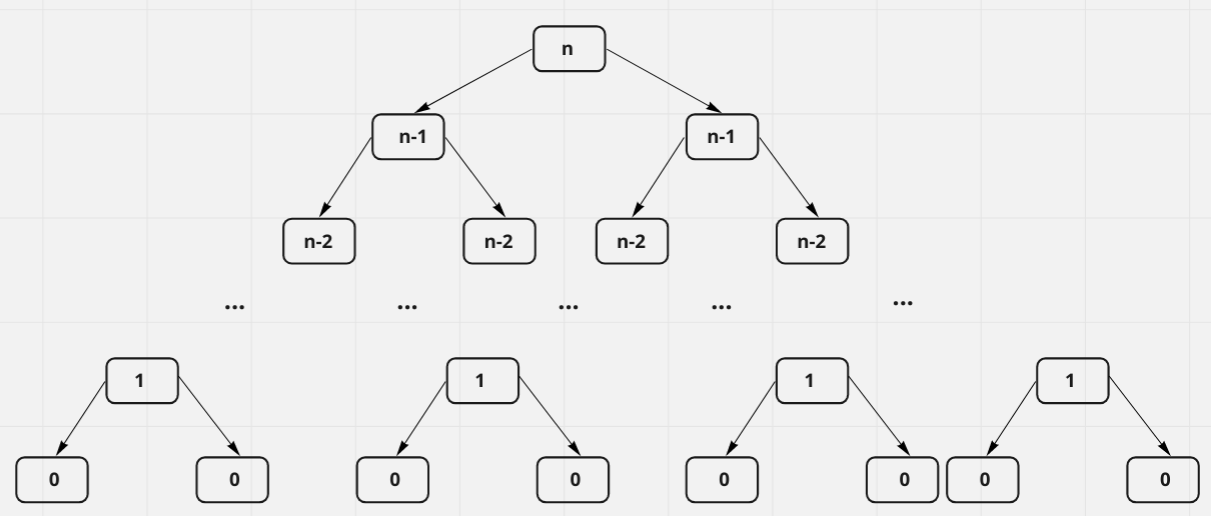
\includegraphics[width=\textwidth]{images/tree.png}
		\end{figure}
	
		Considerando a altura da árvore como $h$, então o número de chamadas seria $2^h$.		
		
		\item Este é um bom algoritmo para resolver este problema.
		
		Para grande entrada, ele não é bom, uma vez que a árvore cresceriam muito. Poderia utilizar um acumulador a cada iteração e somando o número 2 $n$ vezes. Isso poderia melhorar a eficiência do algoritmo.		
	\end{enumerate}

	\item Considere o seguinte algoritmo recursivo:
	
	\begin{enumerate}
		\item O que este algoritmo faz?
		
		Encontra o menor elemento do \textit{array}.
		
		\item  Apresente a relação de recorrência para a operação básica do algoritmo, conte o número de operações, resolva a relação.
		
		$C(n) = C(n-1)+1,$ para $n>1$, $A(1)=0$
		
		\begin{table}[H]
			\centering
			\begin{tabular}{ccl}
				$C(n)$ & $=$ & $C(n-1)+1$\\
				$C(n)$ & $=$ & $[C(n-2)+1]+1=C(n-2)+2$\\
				$C(n)$ & $=$ & $[C(n-3)+1]+2=C(n-3)+3$\\
				$C(n)$ & $=$ & ...\\
				$C(n)$ & $=$ & $C(n-i)+i$\\
				$C(n)$ & $=$ & ...\\
				$C(n)$ & $=$ & $n-i=1 \rightarrow i=n-1$\\
				$C(n)$ & $=$ & $C(1)+(n-1) = n-1$\\
			\end{tabular}
		\end{table}				
	\end{enumerate}

	Logo, o número de operações é igual a $n-1$.
	
	\item Quais são os limites da análise matemática de algoritmos? Qual a alternativa?
	
	A análise matemática pode ser aplicada muita das vezes na maioria dos algoritmos, porém há alguns casos, algoritmos simples, que a precisão matemática torna-se difícil de ser analisada, principalmente na análise de casos médio. Outro limite também seria a limitação em relação as fórmulas aplicadas na resolução de relações de recorrências, a dificuldade de cálculos em \textit{loops} irregulares e não levar em consideração o tipo de entrada mas sim o tamanho da entrada. Apesar de não depender das entradas, sua aplicabilidade é limitada. Uma alternativa seria a análise empírica que é utilizada para comparar eficiência de vários algoritmos que resolvem o mesmo problema ou diferentes implementações do mesmo algoritmo.	
	
	
	\item Resuma o processo de análise empírica de algoritmos, descrito na seção 2.6 do Capítulo 2 do livro \textit{Introduction to the Design and Analysis of Algorithms (3rd Edition) - Anany Levitin}.
	
	A análise empírica segue um plano.Para medir a eficiência de um algoritmo pode implementar uma das alternativas: contar o número de vezes que a operação básica foi executada ou medir o tempo de execução do algoritmo (comando time em UNIX, por exemplo). Um dos problemas é que o tempo de execução dos sistemas não são muito acurados uma vez que normalmente o tempo informado considera o tempo compartilhado com outros programas e não apenas o programa em questão.\\
	Depois de decidir a métrica (tempo de \textit{clocking} ou número de vezes de execução da operação básica), escolhe-se um conjunto de entrada para o experimento. Não um conjunto pronto e especifíco para cada algoritmo, logo o analisador terá que criar seu próprio conjunto. Um dos cuidados é o tamanho da amostra de entrada. Não pode seguir um padrão nem ser randômica.  
	Depois de escolhida as entradas, executa-se o algoritmo com essa entrada e armazena os resultados para análises futuras. Pode-se utilizar uma tabela ou um recurso gráfico como o \textit{scatterplot}. 
	Outro uso da análise empírica está no uso da predição de performance de instâncias que não estavam presentes no conjunto de entradas. Apesar da versatilidade do uso deste tipo de análise, a dependência de um conjunto de entradas e da máquina que executa o algoritmo enfraquece um pouco essa técnica de análise.
	
	
	\item Considere o algoritmo abaixo que verifica se um grafo, definido por sua matriz de adjacência é completa. Qual é classe de eficiência deste algoritmo no pior caso?
	
	$C(n)= C(n-1)+n-1$ para $n>1, C(1)=0$
	
	\begin{table}[H]
		\centering
		\begin{tabular}{ccl}
			$C(n)$ & $=$ & $C(n-1)+n-1$\\
			$C(n)$ & $=$ & $[C(n-2)+n-2]+n-1=C(n-2)+(n-2)+(n-1)$\\
			$C(n)$ & $=$ & $[C(n-3)+n-3]+(n-2)+(n-1)=C(n-3)+(n-3)+(n-2)+(n-1)$\\
			$C(n)$ & $=$ & ...\\
			$C(n)$ & $=$ & $C(n-i)+(n-i)+(n-i+1)+(n-i+2)+(n-i+3)+...+(n-1)$\\
			$C(n)$ & $=$ & ...\\
			$C(n)$ & $=$ & $n-i=1 \rightarrow i=n-1$\\
			$C(n)$ & $=$ & $C(1)+1+2+3+4+...+(n-1) = 0+1+2+3+4+...+(n-1)=\dfrac{n(n-1)}{2}$\\
		\end{tabular}
	\end{table}	
		
\end{enumerate}


\bibliography{bib/refer.bib}

\end{document}
